\documentclass{article}
\usepackage{amsmath} 
\usepackage{graphicx} 
\usepackage{authblk}
\usepackage{url}
\usepackage{hyperref}
\usepackage{multirow}
\usepackage{amssymb}
\usepackage[linesnumbered,boxed]{algorithm2e}

\topmargin 0.0cm
\oddsidemargin 0.2cm
\textwidth 16cm 
\textheight 21cm
\footskip 1.0cm

\title{Quantum Monte Carlo method and and Its Application in Physics}
\author{Mengzhi Chen}
\affil{Department of Physics and Astronomy, Michigan State University}
\date{}

\begin{document}
	\maketitle
	\begin{abstract}\label{abstract}
Monte Carlo (MC) method is widely used in scientific computations.
This method relies on huge amount of random samplings to obtain numerical results.
MC method shows high efficiency and precision when dealing with many complex problems, such as non-analytic and high demential integrals. 
In this report we apply MC method together with variational principle to calculate the ground state energy of two electrons moving in a harmonic oscillator(H.O.) potential.
We assumed two forms of trial wave functions with parameters. 
By using MC method, we find their optimistic parameters corresponding to ground state energies.
The agreements with results from diagonalization method (in Project 2) validate our MC simulations.
We also test the virial theorem for different relative strength between H.O. potential and Coulomb repulsion.

	\end{abstract}

\section{Introduction}\label{intro} 
The initial value problem often appears in physics, especially in Newtonian mechanics. 
Applying Newton's second law on a $n$-body system with no external force, we obtain the equations of motion 
\begin{equation}\label{eq:newton}
m_i\frac{d^2\vec{r}_i}{dt^2}=\sum_{j=1,\ j\neq i}^{n}\vec{F}_{ij},\ i=1,2,\cdots n, 
\end{equation}
where $m_i$, $\vec{r}_i$ and $\vec{F}_{ij}$ are the mass of object $i$, coordinate of object $i$ 
and force between object $i$ and $j$, respectively. 
Here we have $\vec{F}_{ij}=-\vec{F}_{ji}\ (i\neq j)$. 
Eq. \ref{eq:newton} can be transformed into a set of first-order differential equations: 
\begin{equation}\label{eq:firstorder}
	\left\{  
	\begin{array}{lr}  
	\vec{v}_i=\frac{d\vec{r}_i}{dt} \\
	\frac{d\vec{v}_i}{dt}=\frac{1}{m_i}\sum_{j=1,\ j\neq i}^{n}\vec{F}_{ij} 
	\end{array}  
	\right. 
	\ i=1,2,\cdots n, 
\end{equation}
where $\vec{v}_i$ is the velocity of object $i$. 
Eq. \ref{eq:firstorder} should be solved with specified initial $\vec{r}_i$ and $\vec{v}_i$, namely 
\begin{equation}
	\left\{  
	\begin{array}{lr}  
	\vec{r}_i(t_0)=\vec{r}^{(0)}_i \\
	\vec{v}_i(t_0)=\vec{v}^{(0)}_i
	\end{array}  
	\right. 
	\ i=1,2,\cdots n, 
\end{equation}
where $t_0$ is the initial time (usually $t_0=0$). 
\par
In the history of physics, the great success of Newtonian mechanics was partly from 
its (almost) perfect explanation of planets' motion in the solar system. 
Eq. \ref{eq:newton} of a two-body system with gravity has an analytical solution, 
which gives a conic section orbit. 
However, a $n$-body ($n>2$) system with gravity cannot be solved analytically, 
making it necessary to explore the numerical methods for the initial value problem. 
In Sec. \ref{physcis_problem} we will give the equations for both two- and many-body systems with gravity, 
and discuss two numerical methods (Euler's forward and Velocity-Verlet methods) in Sec. \ref{method}. 
Sec. \ref{results} will discuss and compare the results of applying
these two methods on the Earth-Sun, Earth-Sun-Jupiter and whole solar system. 

\section{A physicical system}\label{phys}
A simple physical system we studied is two electrons confined in a three dimensional H.O. potential. 
It's Hamiltonian (in atomic unit (a.u.)) has three parts
\begin{equation}
	\hat{H}=\sum_{i=1,2}(-\frac{1}{2}\nabla_i^2+\frac{1}{2}\omega^2r_i^2)+\frac{1}{r_{12}},
\end{equation}
where two in parenthesis are their kinetic and potential energies, third is the Coulomb repulsion between electrons. 
The first trail wave function we used is 
\begin{equation}\label{eq:t1}
	\Phi_{t1}(\vec{r}_1,\vec{r}_2)=C\rm{exp}(-\alpha \omega (\vec{r}_1+\vec{r}_2)/2)
\end{equation}
which simply the product of two electrons' wave functions in H.O. potential without repulsion.
The $C$ works for normalization and $\alpha$ is the only one variational parameter here.

One step further, in order to get rid of divergence when $r_{12}\rightarrow 0$, we have second trail wave function
\begin{equation}\label{eq:t2}
	\Phi_{t2}(\vec{r}_1,\vec{r}_2)=C\rm{exp}(-\alpha \omega (\vec{r}_1+\vec{r}_2)/2)\rm{exp}(\frac{r_{12}}{2(1+\beta r_{12})})
\end{equation}
which satisfies the cusp condition.
In this $\Phi_{t2}$ we add an extra term called Jastrow factor.
And now, it has two variational parameters $\alpha$ and $\beta$.
Substituting these two trail wave functions to \ref{local}, we can obtain their local energies
\begin{equation}
	E_{L1}= \frac{1}{2}\omega^2(\vec{r}_1^2+\vec{r}_2^2)(1-\alpha ^2)+3 \alpha \omega + \frac{1}{r_{12}}
\end{equation}
\begin{equation}
	E_{L2}= E_{L1}+\frac{1}{2(1+\beta r_{12}^2)}\left( \alpha \omega r_{12}-r_{12}^2-\frac{2}{r_{12}}+\frac{2\beta}{1+\beta r_{12}}\right).
\end{equation}
We can see the second local energy is much complicated than the first one with the help of the Jastrow factor. 
We will see whether it worthwhile to pay this extra price from our results.

	
	
\section{Numerical methods}\label{method}
	\subsection{Metropolis algorithm}\label{metro}
	Sampling strategy is the crucial part in a MC simulation.
Metropolis algorithm solves the problem of sampling from a targeted complex distribution.
Before introducing this algorithm, we first need to understand the Markov chain and transfer matrix.
A Markov chain together with a transfer matrix $P$ describe evolution of a system from initial $\pi_0(x)$ to equilibrium $\pi(x)$.
$\pi_i(x)$ is status at moment $i$ and it only relies on previous status $i-1$ by $P$
\begin{equation}
	\pi_i(x)=\pi_{i-1}(x)P = ... = \pi_0(x)P^i
\end{equation}
At equilibrium, we have 
\begin{equation}
	\pi_n(x)=\pi_{n-1}(x)P = ... = \pi(x)
\end{equation}
Practically, we often know the information of equilibrium $\pi(x)$. 
However, it's hard to obtain how system evolves as $P$ which prevents our direct sampling.
In this situation, we need the help of Metropolis algorithm. 

At equilibrium, the system has detailed balance condition
\begin{equation}\label{detail}
	\pi(i)P(i,j)=\pi(j)P(j,i).
\end{equation} 
This condition is not valid for a random transfer matrix $Q$.
In Metropolis algorithm, we introduce an acceptance probability $\alpha(i,j)=P(i,j)Q(j,i)$, so Eq. \ref{detail} can be fulfilled as
\begin{equation}\label{detail}
	\pi(i)Q(i,j)\alpha(i,j)=\pi(j)Q(j,i)\alpha(j,i).
\end{equation} 
for any $Q$ we used.
Then, the aimed transfer matrix $P(i,j)=Q(i,j)\alpha(i,j)$

\begin{algorithm}[tb]
	\caption{Metropolis algorithm}
	\label{alg::metro}
	\KwIn{transfer matrix $Q$, equilibrium $\pi(x)$ }
	\KwOut{samples ($x_{n1},x_{n1+1},...,x_{n1+n2-1}$)} 
    // Sampling from n1 to n1+n2-1\;
    \For{$i=0;i<n1+n2-1;i++$}
    {Taking sample from $Q(x^{\ast}|x_i)$\;
    Taking $u$ ~ uniform[0,1]\;
    \If{u$< \pi(x^{\ast})*Q$}
    {
    accept transfer $x_{i+1}=x^{\ast}$
    }
    Otherwise $x_{i+1}=x_{i}$
    }
	return ($x_{n1},x_{n1+1},...,x_{n1+n2-1}$)\;
\end{algorithm}

The flow of Metropolis algorithm is shown is Alg. \ref{alg::metro}. 
In a word, we can approximate an unusual distribution from a usual one through acceptance and rejection with certain probabilities.

	
	\subsection{Variational Monte Carlo(VMC) method} \label{vmc}
	The idea of Metropolis algorithm is also suitable in  variational MC calculation.
As shown in Alg. \ref{alg::vmc}, starting from given variational parameters and trail wave function, we move the sampling point randomly.
Also, we accept or reject this movement according to $P_L$.

It worth noticing that the movement step size is adjusted to obtain about $50\%$ acceptance. 
High acceptation can trap movement locally which means a low accuracy; a low acceptation means a large waste of sampling points.
So, it's a trade-off between accuracy and efficiency.

\begin{algorithm}[tb]
	\caption{Variational MC method}
	\label{alg::vmc}
	\KwIn{$\alpha,\beta, \omega$, $\Phi_{t}$, $E_L$,$P_L$}
	\KwOut{($E_L(n1),E_L(n1+1),...,E_L(n1+n2-1)$)} 
    // Sampling from n1 to n1+n2-1\;
    // Initiate random starting position $r_1(0),r_2(0)$ \;
    \For{$i=0;i<n1+n2-1;i++$}
    {$r_1(i) = r_1(i-1)+step*r, r_2(i) = r_2(i-1)+step*r$ ($r$ ~ uniform[0,1])\;
    Taking $u$ ~ uniform[0,1]\;
    \If{u $ < P_L(i)/P_L(i-1)$}
    {
    accept movement $r_{i}=r_{i}$\;
    }
    Otherwise $r_{i}=r_{i-1}$\;
    }
    //Calculate $E_L,E_L^2 $\;
	return ($E,\sigma$)\;
\end{algorithm}



	
\section{Results and discussions}\label{results}

	\subsection{First trail wave function}
	In our first calculation, we take the first trail wave function \ref{eq:t1}.
At beginning, we take $\omega=1.0$ and vary $\alpha$ from 0.675 to 1.15.
The total number MC samplings $N$ is set to be $10^7$.
\begin{figure}[tb]
\label{fig:t1}
\centering
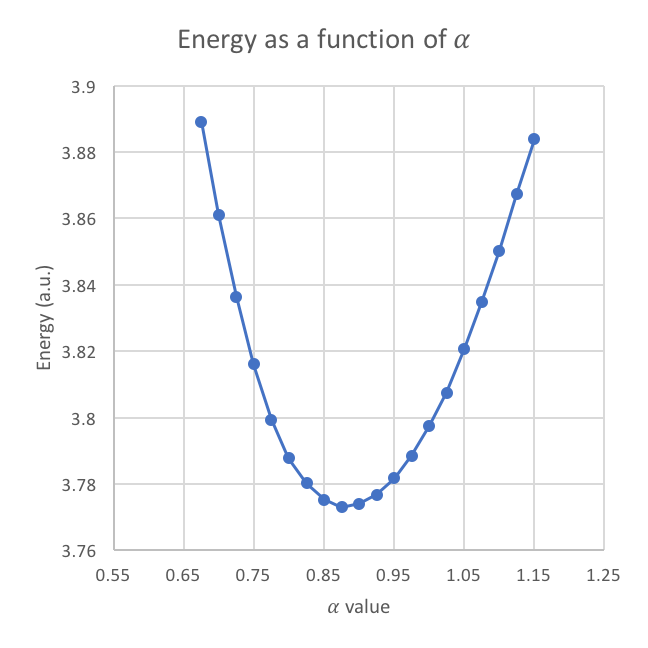
\includegraphics[width=0.4\textwidth]{t1.png}
\caption{Relation between lowest $E$(a.u.) and the variational parameter $\alpha$ where $\omega$ is set to one and $N=10^7$ obtained from $\Phi_{t1}$.}
\end{figure}

In Fig. \ref{fig:t1}, we show lowest energies for different $\alpha$. 
Clearly, it has a minimum value $E_{min}=3.7729\ a.u.$ corresponding to $\alpha=0.875$.
Energies and variances for some $\alpha$ are shown in Table \ref{tab:t1}.
We can see that the accuracy can be improved by sample more points ($N$).
\begin{table}[tb]
	\centering
	\caption{Lowest energies and variances for   different $\alpha$ (partly) where $\omega$ is set to one and $N=10^7$ obtained from $\Phi_{t1}$. All qualities are in atomic unit.}
	\label{tab:t1}
	\begin{tabular}{cccc}
		\hline
		\hline
		$\alpha$   & E & $\sigma^2$ & $\sigma/\sqrt{N}$ \\
		\hline
		0.75 &3.8161 &0.3285 &5.731E-04 \\
		0.85 &3.7753 &0.2715 &5.211E-04 \\
		0.95 &3.7817 &0.3085 &5.554E-04 \\
		1.05 &3.8207 &0.4264 &6.530E-04 \\
		1.15 &3.8839 &0.5968 &7.725E-04 \\
		\hline
		\hline
	\end{tabular}
\end{table}
In next step, we fixed $\alpha=0.875$ which is optimal value and change $\omega$ to 0.01 and 0.5.
We calculate the expectation value of distance between to electrons $r_{12}$. 
The results are listed in the second column of Table \ref{tab:t12}.
It shows that $r_{12}$ increases as decreasing $\omega$.
The reason for that is simple.
A smaller $\omega$ means a weaker H.O. potential which can not trap electrons tightly, so they repel each other to reach a larger $r_{12}$.
\begin{table}[tb]
	\centering
	\caption{Relations between $\omega$ and $r_{12}$ where $\alpha$ is set to 0.875 and $N=10^7$. The second column is calculated from $\Phi_{t1}$ and third from $\Phi_{t2}$. All qualities are in atomic unit.}
	\label{tab:t12}
	\begin{tabular}{ccc}
		\hline
		\hline
		$\omega$   & $r_{12}(t1)$ &$r_{12}(t2)$ \\
		\hline
		0.01 &17.0726 &18.636  \\
		0.50 &2.4137 &2.6774  \\
		1.00 &1.7074 &1.828  \\
		\hline
		\hline
	\end{tabular}
\end{table}



	\subsection{Second trail wave function}
	As mentioned before, we add the Jastrow term to form the second trail wave function Eqt. \ref{eq:t2}.
Moreover, in this situation, we have two variational parameters $\alpha$ and $\beta$.
It largely increases our computing time.

This time, we still start from $\omega=1$ and $N=10^7$ and vary $\alpha$ from 0.675 to 1.15, $\beta$ from 0.1 to 0.3.
Here, it will be cumbersome to show all energies and variances.
So we only present a Fig. \ref{fig:t2} to give an intuitive impression.
\begin{figure}[tb]
\label{fig:t2}
\centering
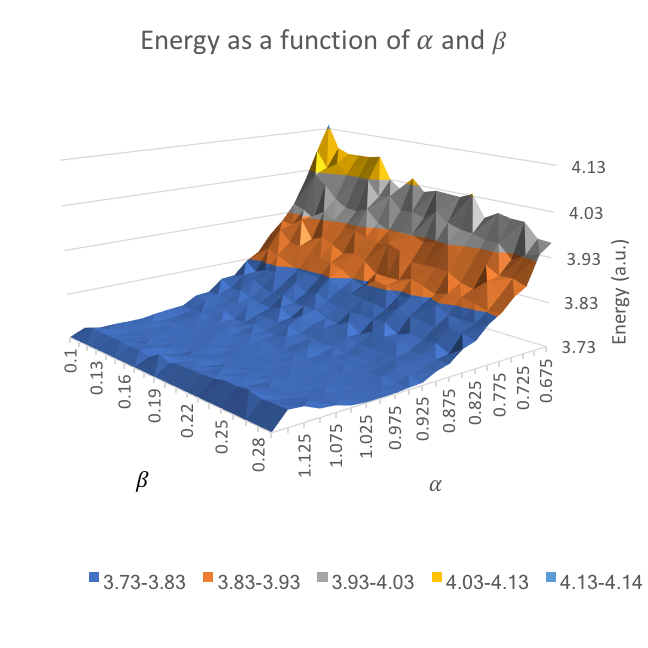
\includegraphics[width=0.4\textwidth]{t2.png}
\caption{Relation between lowest $E$(a.u.) and the variational parameters $\alpha$ and $\beta$ where $\omega$ is set to one and $N=10^7$ obtained from $\Phi_{t2}$.}
\end{figure}
The lowest energy is $E_{min}=3.7305\ a.u.$ with parameters $\alpha=1.025$ and $\beta=0.18$.
The $r_{12}$ obtained from $\Phi_{t2}$ are listed in the third column of Table \ref{tab:t12}.
We can see the values are larger than the second column (from $\Phi_{t1}$).
It is reasonable because $\Phi_{t1}$ doesn't take Coulomb repulsion into account in the wave function.
It then underestimates the distance $r_{12}$.

In project 2, we also solve the ground state energy of this system by diagonalizing its Hamiltonian.
It gives a rather accurate results for this system.
So we use it as a standard benchmark of results obtained from MC method.
\begin{table}[tb]
	\centering
	\caption{Minimum energies calculated from two trail wave functions (second and third columns) and diagonalization method (fourth column). Optimal parameter used with $\omega=0.01,0.5$ and 1.0, $N=10^7$. All qualities are in atomic unit.}
	\label{tab:diag}
	\begin{tabular}{cccc}
		\hline
		\hline
		$\omega$   &$E_{min}(t1)$ & $E_{min}(t2)$ & $E_{min}(diag)$ \\
		\hline
		0.01 &0.104 &0.0935 &0.0796  \\
		0.50 &2.0394 &2.0005 &1.99995  \\
		1.00 &3.7729 &3.7305 &3.72992 \\
		\hline
		\hline
	\end{tabular}
\end{table}
Their results are shown in Table \ref{tab:diag}.
We can see both second and third columns obtained by MC method for two different trail wave functions  reproduce results from diagonalization method.
Deviations are larger for $\omega \neq 1$ because we keep using optimal parameters for $\omega=1$ which is not the best for other .
Furthermore, $\Phi_{t2}$ gives smaller error than $\Phi_{t1}$ which means the Jastrow factor makes it more similar to exact the wave function.


	
	\subsection{Test of virial theorem}
	The virial theorem tells us the relation between expectation values of kinetic $<T>$ and potential energy $<V>$.
For two special interactions, H.O. potential and Coulomb repulsion.
The relations are
\begin{equation}\label{eq:virial}
	<T>=<V>\ (\rm{H.O.})
\end{equation}
\begin{equation}
	<T>=\frac{1}{2}<V>\ (\rm{Coulomb})
\end{equation}
Both these two interactions exist in our system, so the ratio between $<T>$ and $<V>$, where we defined as $\chi$ should locates between 0.5 and 1.
The $\chi$ value is determined by relative strength between these two interactions.

In our calculations, we consider two situations using 
the first trail wave function $\Phi_{t1}$.
One without Coulomb interaction then $\alpha=1.0$, as expected, because it's a product of two free electrons' wave functions.
The other with Coulomb interaction has different value of optimal $\alpha$ for different  $\omega$. 
We vary $\omega \in [0.01,1]$ to control relative strength between H.O. potential and Coulomb repulsion and calculate the value of $\chi$.
\begin{figure}[tb]
\label{fig:virial}
\centering
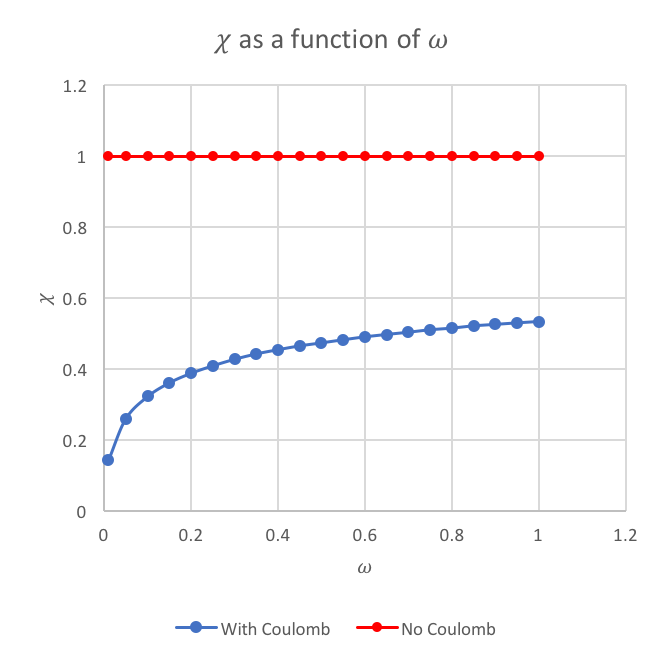
\includegraphics[width=0.4\textwidth]{virial.png}
\caption{Relation between lowest $E$(a.u.) and the variational parameters $\alpha$ and $\beta$ where $\omega$ is set to one and $N=10^7$ obtained from $\Phi_{t2}$.}
\end{figure}
The results are shown in Fig. \ref{fig:virial}.
The red curve is the one without Coulomb repulsion.
It gives a trivial result follows Eqt. \ref{eq:virial}.
For the blue curve represents situation with Coulomb repulsion.
As expected, We can see $\chi$ growths with increasing $\omega$ which indicates stronger H.O. potentials.
However, its value doesn't locate in 0.5 and 1. 
My suggestion for this problem is on trail wave function $\Phi_{t1}$ we used.
It has a form of free electron in H.O. potential, so it deviates a lot from exact one especially for weak H.O. potentials (small $\omega$).


	
\section{Conclusions}\label{conclude}
	In this report, we introduce MC method and Metropolis algorithm which can be used to calculate integrals.
To study two electrons confined in a H.O. potential, we combine MC method with variational principle.
We use two different trail wave functions in our calculations.
The first one $\Phi_{t1}$ is a product of two electrons in H.O. potential wave functions with one parameter.
The second $\Phi_{t2}$ has two parameters by adding the Jastrow factor to correct behavior when electrons get very close.
We find optimal parameters and ground state energies for these two trail wave functions.
By comparing with results given by diagonalization method, validity of MC method is proved.
Moreover, $\Phi_{t2}$ gives better results than $\Phi_{t1}$ which justifies the power of the Jastrow factor.
In last step, we test the virial theorem using $\Phi_{t1}$ by adjusting the relative strength of H.O. potential and Coulomb repulsion.
The curves give right trends as expected.
	
	\section*{Acknowledgments}
	We are grateful for the sincere guidance from Prof. Morten Hjorth-Jensen. 
	
	\nocite{*} 
	\bibliographystyle{unsrt}
	\bibliography{proj4_ref}
\end{document}